IBM erm\"oglicht durch ihre Onlineplattform IBM Quantum \cite{IBM_Quantum} den Zugang zu reelen Quantencomputern oder zu simulierten Quantencomputern auf Leistungsf\"ahiger Hardware. IBM Quantum bietet durch das Werkzeug Quantum Composer einen einfachen Einstieg in den Bereich der Quantencomputer f\"ur Neueinsteiger. Quantum Composer erm\"oglicht durch Ziehen und Ablegen \textit{(Drag and Drop)}, Quantenschaltungen aufzubauen. Auch vorgefertigte Schaltungen/Algorithmen werden angeboten und k\"onnen vom Benutzer ausgef\"uhrt, ver\"andert und angepasst werden. Auf Grundlage dieser Schaltungen wird Code generiert, dieser kann falls n\"otig vom Benutzer beliebig ver\"andert und angepasst werden.
\begin{figure}[h]
\centering
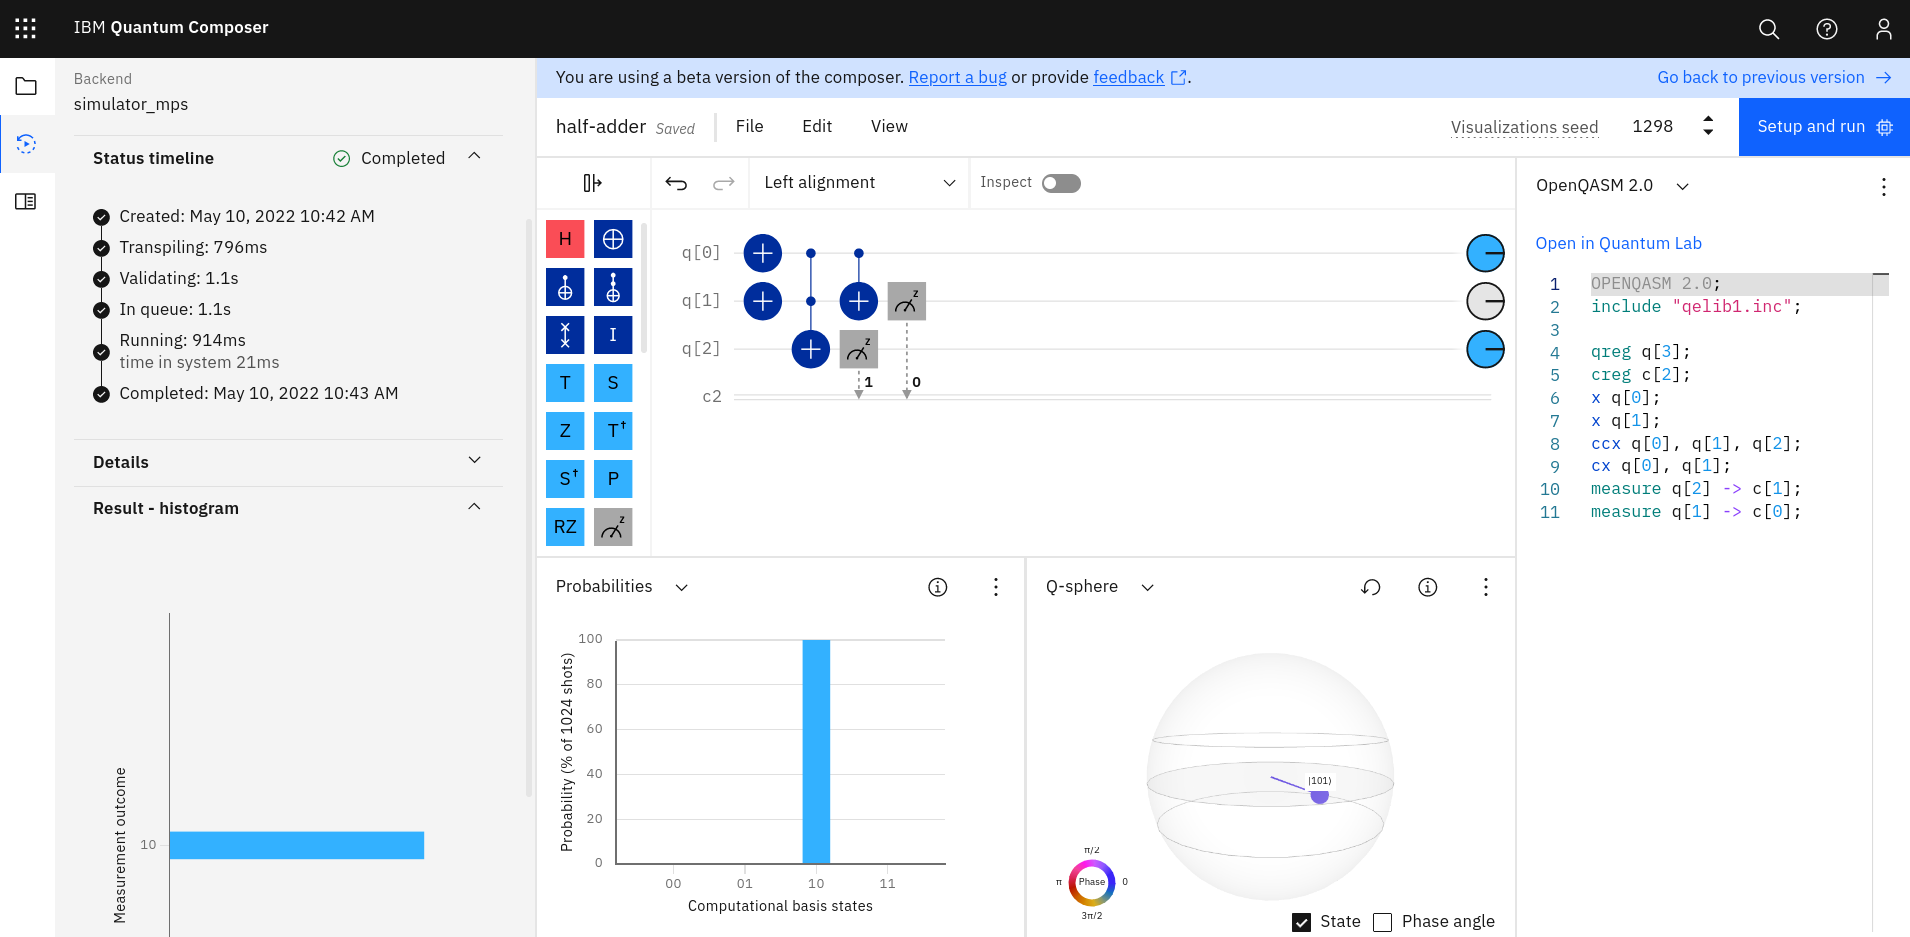
\includegraphics[width=1\textwidth]{figures/half_adder_composer.png}
\caption{Quantum-Halbaddierer simuliert auf den \textit{simulator_mps}}
\label{fig:quantum-composer}
\end{figure}
Abbildung \ref{fig:quantum-composer} zeigt die Oberfl\"ache des Quantum Composers. N\"ordlich kann der Benutzer die erstellte Schaltung sehen und bearbeiten. S\"udlich des Bildes kann die Wahrscheinlichkeit der Ausgabe sowie dessen Zustand innerhalb der Q-Kugel betrachtet werden. \\\\
Die Ausf\"uhrung dieser Schaltung bzw. dieses Programms auf einem realen Quantencomputer, oder die Simulation auf einem HPC \textit{(High Performance Computer)} in der Cloud, wird durch den IBM Quantum Service ausgef\"uhrt. Der IBM Quantum Service bezeichnet diese Schaltungen als Jobs und verwaltet diese durch einen kubernetes Cluster. Dieses Cluster beinhaltet einen Runtime Manager, Runtime Job und einen Execution Kernel.\\\\
Fortgeschrittene Benutzer haben durch das Quantum Lab und Qiskit die M\"oglichkeit in der Cloud Juypter-Notebooks zu verfassen. Durch die quelloffenen Programmierschnittstelle \textit{(API)} Qiskit, wird es erm\"oglicht Quantencomputer auch lokal auf Ebene von Schaltungen und Algorithmen zu programmieren. Dabei m\"ochte Qiskit eine standardisierte API entwickeln, die f\"ur verschiedenste Benutzergruppen geeignet ist \cite{Qiskit_backend_2018}. Um Schaltungen auf unterschiedlicher Hardware interpretieren lassen zu k\"onnen, werden die in Qiskit erzeugten Objekte von JSON zu OpenQASM umgewandelte. OpenQASM ist dabei jedoch keine Ausgangssprache oder die Instruktionen einer Zielmaschine, sondern eine Zwischendarstellung \textit{(intermediate representation (IR))} \cite{Openqasm_2017}. In Anhang \ref{chap:anhang} wird der Code eines Quanten-Halbaddieres in Qiskit und OpenQASM dargestellt.

